\documentclass[12pt,a4paper]{article}
\usepackage[latin1]{inputenc}
\usepackage{amsmath}
\usepackage{amsfonts}
\usepackage{amssymb}
\usepackage{graphicx}
\usepackage{float}
\usepackage{gensymb}
\usepackage{hyperref}
\usepackage{cite}
\usepackage[margin=1in]{geometry}
\usepackage[justification=centering, font={small,it}]{caption}
\author{Dicson Wijaya (1002289), Wenkie Lau (1002219), \\ Mok Jun Neng (1002219), Charlotte Phang (1002277), \\ Martin Tan (1002173)}
\title{Systems World 2D Question 3\\ F06 Team 06}

\begin{document}
	\maketitle
	\section{Part (a)}
	The $\chi^2$ goodness of fit test will be used as a continuation of Question 2.
	To formulate this as an optimisation problem, the objective would be to:
	\begin{enumerate}
		\item Maximise the number of zero coefficients ($k_i$)
		\item Minimise the $\chi^2$ value of the $m$\textsuperscript{th} order controller.
	\end{enumerate} 
	In other words, as two conflicting objective functions will have to be optimised, a compromise has to be found based on a maximum predetermined value of $\chi^2$. This value of $\chi^2$ will correspond to a significance level $\alpha$ that is acceptable for the goodness of fit, where $\alpha = P($Reject $H_0|H_0$ is true$)$.\\
	
	For the null hypothesis: $\{H_0$: The $m$\textsuperscript{th} order controller fits the measured data$\}$, $\alpha$ would be set to $0$ in the ideal case. However, it is a mathematical fallacy to set $\alpha = 0$ as it is always possible to find an exact solution solution for 10 unknowns ($k_i$ values) given a 9\textsuperscript{th} order controller (which gives a system of 10 equations). Hence, prior to analysing the data, the significance level $\alpha$ is set to $0.001$. In order to minimise the number of non-zero coefficients ($k_i$), we introduce a binary switch $x_i$.\\
	
	Modifying the objective function in question 2, we have: \\
	$$\min \sum_{n=0}^{9} \bigg( \sum_{i=0}^{9} \frac{(k_i x_i e(n-i) - v(n))^2}{v(n)} \bigg) + \sum_{i=0}^{9} x_i$$
	
	Constraints: 
	$$x_{1,2,3...n} \ \epsilon \ \{ 0,1 \}$$
	\begin{center}$(\chi^2$ test p-value$) \ <0.001$\end{center}
	
	Decision Variables: 
	$$x_{1,2,3...n} \ , \ k_{1,2,3...n}$$
	
	Parameters: 
	$$e(n) \ , \ v(n); \ \forall n \in \lbrack 1, \ 9 \rbrack $$
	
	\section{Part (b)}
	From question 2, a chi-square distribution with 9 degrees of freedom for a lower one-sided test at significance level $\alpha = 0.001$ has a critical value of 1.152. Therefore, a constraint that has to be set is to have the $\chi^2$ value to be less than or equal to the critical value 1.152. This constraint is equivalent of setting a constraint on the p-value $<0.001$, and sets the ceiling or upper bound for the objective function.
	\begin{figure}[H]
		\begin{center}
			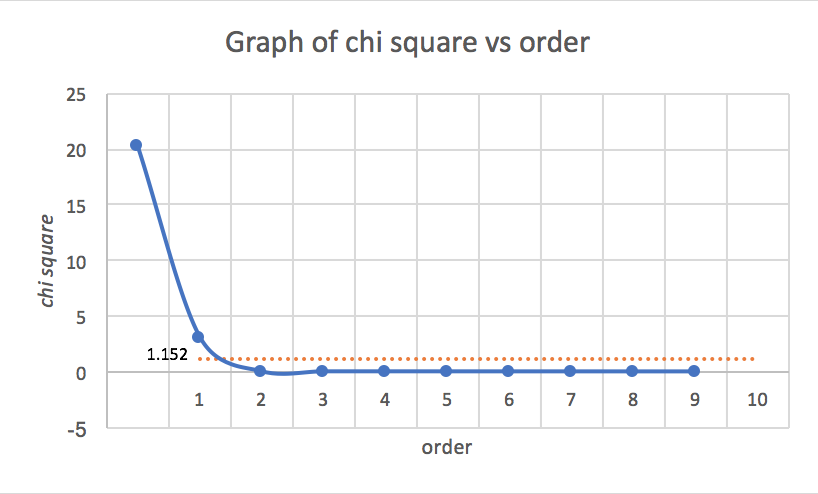
\includegraphics[width=0.75\textwidth]{chi.png}
			\caption{Graph of $\chi^2$ values against Order of Controller}
			\label{fig:chi}
		\end{center}
	\end{figure}

	Figure \ref{fig:chi} above shows the minimum attainable values of $\chi^2$ for each order $m$. It can be observed that the order $m = 2$ satisfies the condition $\chi^2 < 1.152$ as shown by the dotted line.\\
	
	From the objective function defined in part (a), an additional binary switch multiplier was included as a decision variable. This results in 10 $\chi^2$ values from each order multiplied by the binary switch. Since we may only choose one value that corresponds to the smallest order controller, we set another constraint: $\sum_i x_i = 1$. Hence, only one chi-square value out of the ten data points, corresponding to the smallest order controller, will appear to be non-zero. Since Excel Solver requires the objective function to be a formula, we simply set it as the sum of chi-square values with the binary switch on. The objective function simply becomes $\sum_{i} \chi^2_i x_i$
	\begin{figure}[H]
		\begin{center}
			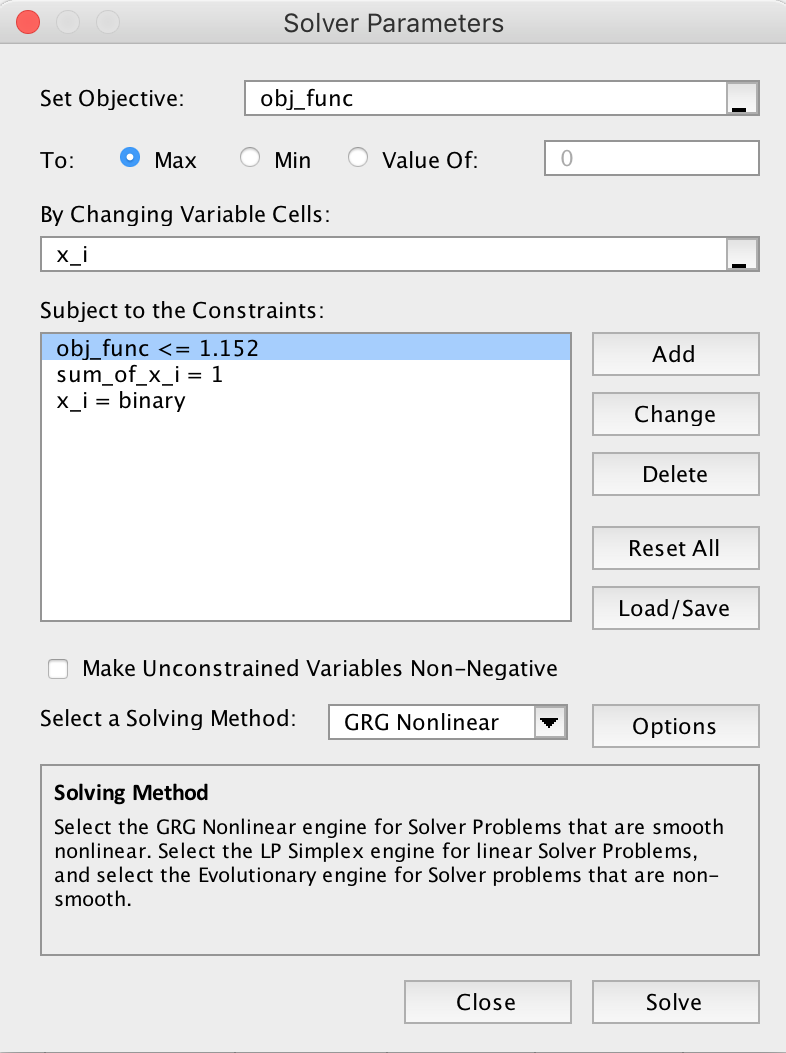
\includegraphics[width=0.7\textwidth]{constraints.png}
			\caption{Constraints to find the objective function in Excel Solver}
			\label{fig:constraints}
		\end{center}
	\end{figure}
    \begin{figure}[H]
    	\begin{center}
    		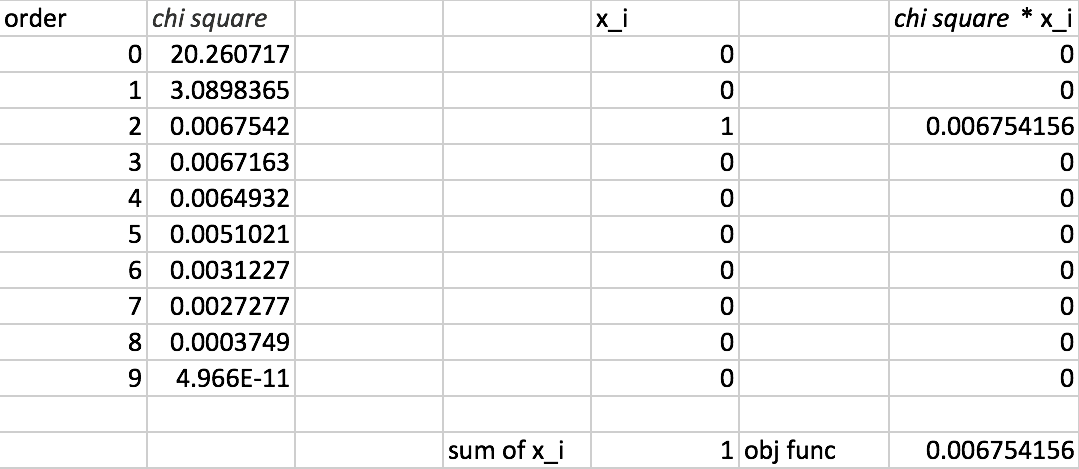
\includegraphics[width=0.75\textwidth]{xcel.png}
    		\caption{Screenshot of Calculations in Microsoft Excel}
    		\label{fig:xcel}
    	\end{center}
    \end{figure}
    Since we have considered all possible orders $m \in \lbrack 0, \ 9 \rbrack$ in maximising the objective function ($m$ cannot be larger than $9$ as there is insufficient data), the only controller that satisfies the constraints is of order $m = 2 \Rightarrow H_0$ cannot be rejected.
	
\end{document}